\documentclass[a4paper,14pt,oneside]{extreport}

\usepackage{fontspec}
\setmainfont{Times New Roman}
\setmonofont{Courier New}
\newfontfamily\cyrillicfonttt{Courier New}
\usepackage{unicode-math}
\setmathfont{STIX Two Math}
\usepackage{polyglossia}
\setdefaultlanguage{russian}
\setotherlanguage{english}
\addto\captionsrussian{\renewcommand{\contentsname}{}}

\usepackage{geometry}
\geometry{left=3cm,right=1.5cm,top=2cm,bottom=2cm}
\renewcommand{\baselinestretch}{1.5}
\setlength{\parindent}{1.25cm}
\setlength{\parskip}{0pt}
\usepackage{microtype}

\usepackage{amsmath}
\usepackage{graphicx}
\usepackage{float}
\usepackage{array}
\usepackage{caption}
\DeclareCaptionLabelSeparator{gost}{~---~}
\captionsetup[lstlisting]{labelsep=gost}
\usepackage{titlesec}
\usepackage{tocloft}
\usepackage{fancyhdr}
\usepackage{tikz}
\usepackage{pgfplots}
\usetikzlibrary{arrows.meta,positioning}
\pgfplotsset{compat=1.18}
\usepackage[htt]{hyphenat}
\usepackage{enumitem}
\setlist[itemize]{label=---,leftmargin=1.25cm,itemsep=0pt,parsep=0pt,topsep=0.5\baselineskip}
\setlist[enumerate]{label=\arabic*),leftmargin=1.25cm,itemsep=0pt,parsep=0pt,topsep=0.5\baselineskip}
\usepackage{listings}
\usepackage{lastpage}
\renewcommand{\lstlistingname}{Листинг}

\DeclareCaptionFont{nohyph}{\hyphenpenalty=10000}
\captionsetup[figure]{labelsep=gost,justification=centering,font={normalsize,nohyph}}
\captionsetup[table]{position=top,labelsep=gost,justification=raggedright,%
  singlelinecheck=false,indent=0pt,skip=4pt,font={normalsize,nohyph}}

\renewcommand{\thesection}{\arabic{section}}
\titleformat{\section}[block]{\bfseries\hyphenpenalty=10000}{\thesection}{0.5em}{}
\titleformat{\subsection}[block]{\bfseries\hyphenpenalty=10000}{\thesubsection}{0.5em}{}
\titlespacing*{\section}{1.25cm}{1.5\baselineskip}{1\baselineskip}
\titlespacing*{\subsection}{1.25cm}{1.5\baselineskip}{1\baselineskip}

\renewcommand{\cfttoctitlefont}{\hfill\bfseries}
\renewcommand{\cftaftertoctitle}{\hfill}
\renewcommand{\cftsubsecindent}{1.25cm}
\renewcommand{\cftsecleader}{\cftdotfill{\cftdotsep}}

\pagestyle{fancy}
\fancyhf{}
\fancyfoot[C]{\thepage}
\renewcommand{\headrulewidth}{0pt}
\fancypagestyle{plain}{\fancyhf{}\fancyfoot[C]{\thepage}\renewcommand{\headrulewidth}{0pt}}

\emergencystretch=3em
\tolerance=2000
\hbadness=10000
\vbadness=10000

\lstset{
  basicstyle=\fontsize{10}{10}\selectfont\ttfamily,
  breaklines=true,
  columns=fixed,
  keepspaces=true,
  showstringspaces=false,
  tabsize=4,
  language=Python,
  numbers=none,
  aboveskip=\baselineskip,
  belowskip=\baselineskip,
  floatplacement=H,
}

\newcommand{\structural}[1]{%
  \clearpage
  \addcontentsline{toc}{section}{#1}%
  {\centering\bfseries #1\par}%
  \vspace{\baselineskip}%
}
\newcommand{\apphead}[2]{%
  \clearpage
  \phantomsection
  \addcontentsline{toc}{section}{ПРИЛОЖЕНИЕ #1. #2}%
  {\centering\bfseries ПРИЛОЖЕНИЕ #1\par}%
  \vspace{0.5\baselineskip}%
  {\centering\bfseries #2\par}%
  \vspace{\baselineskip}%
}

\setcounter{tocdepth}{2}

\begin{document}

\renewcommand{\figurename}{Рисунок}
\renewcommand{\tablename}{Таблица}

\begin{titlepage}
\thispagestyle{empty}
\noindent
\begin{minipage}[t]{0.20\textwidth}
\vspace{0pt}

\includegraphics[width=\linewidth]{figures/emblem.png}
\end{minipage}\hfill
\begin{minipage}[t]{0.78\textwidth}
\centering
\vspace{0pt}
{\fontsize{12}{15}\selectfont
Министерство науки и высшего образования Российской Федерации\\
Федеральное государственное автономное образовательное учреждение\\
высшего образования\\
«Московский государственный технический университет\\
имени Н.~Э.~Баумана (национальный исследовательский университет)»\\
(МГТУ им. Н.~Э.~Баумана)}
\end{minipage}

\vspace{2\baselineskip}
\begin{center}
{\fontsize{13}{16}\selectfont
{\bfseries ФАКУЛЬТЕТ}\\
Информатики и системы управления\\[0.5\baselineskip]
{\bfseries КАФЕДРА}\\
Теоретической информатики и компьютерных технологий (ИУ9)}\\
\vspace{1.5\baselineskip}
{\bfseries КУРСОВАЯ РАБОТА}\\
\vspace{0.5\baselineskip}
НА ТЕМУ:\\
{\bfseries «Программная коррекция оптических искажений в микроскопии»}\\
\end{center}
\vspace{2\baselineskip}
\begin{flushright}
\begin{tabular}{@{}l@{\hspace{0.8cm}}c@{\hspace{0.4cm}}l@{}}
Студент группы ИУ9-52Б &
  \underline{\hspace{3.6cm}} & Афонькин О.~О.\\
 & {\footnotesize (Подпись, дата)} & {\footnotesize (И.О. Фамилия)}\\[1\baselineskip]
Руководитель курсовой работы &
  \underline{\hspace{3.6cm}} & Брагин А.~В.\\
  \underline{\hspace{3.6cm}} & \\
 & {\footnotesize (Подпись, дата)} & {\footnotesize (И.О. Фамилия)}\\
\end{tabular}
\end{flushright}
\vfill
\begin{center}
Москва 2026~г.
\end{center}
\end{titlepage}
\setcounter{page}{2}
\structural{АННОТАЦИЯ}

При выполнении курсовой работы было разработано программное обеспечение автоматической коррекции хроматических искажений фотографий, сделанных в микроскопии. Искажения описываются тремя компонентами: радиально-аффинным полем поперечных смещений цветовых каналов, продольной расфокусировкой каналов и остаточной цветной каймой у контрастных границ.
Конвейер состоит из геометрической регистрации каналов, опциональной
компенсации продольной аберрации и подавления каймы. Были реализованы следующие стадии: калибровка
по точечной мишени, слепой режим без калибровочного кадра, графический
интерфейс, а также пакетная обработка из командной строки. Эксперименты были проведены
на одиннадцати реальных снимках, включая контрольные; проверены сходимость
повторных прогонов и зависимость времени обработки от разрешения.

Объём работы: \pageref{LastPage}~с., \textbf{6}~рисунков,
\textbf{6}~таблиц, \textbf{4}~приложения, \textbf{14}~источников.

\clearpage
{\centering\bfseries СОДЕРЖАНИЕ\par}
\vspace{\baselineskip}
{\linespread{1}\selectfont\tableofcontents}
\clearpage

\structural{ВВЕДЕНИЕ}

Оптическое стекло преломляет каждую длину волны по-своему, поэтому лучи
собираются в разных точках. В изображении
это вызывает цветные ореолы и двоение контуров, которые наиболее видны на краях поля
зрения~[1, 2, 3]. В микроскопии искажение ухудшает количественные измерения:
сдвиг каналов на несколько пикселей меняет размеры объектов и координаты
меток, размытие канала уменьшает контраст тонких структур. Оптическое решение
--- апохроматические объективы --- существенно повышает стоимость системы, поэтому
программная коррекция по оцифрованному изображению остаётся востребованной.

\textbf{Цель работы} --- разработка программного обеспечения для
автоматической коррекции искажений фотографий в микроскопии.

\textbf{Задачи:}
\begin{enumerate}
\item построить математическую модель латеральной, продольной и остаточной
цветовой составляющих искажения;
\item реализовать калибровку объектива по точечному кадру с оценкой
остаточных смещений;
\item реализовать слепую оценку поля смещений по самому снимку;
\item реализовать подавление остаточной цветной каймы;
\item реализовать компенсацию продольной аберрации;
\item разработать графический интерфейс и пакетную обработку;
\item измерить зависимость времени обработки от разрешения.
\end{enumerate}

\textbf{Объект исследования} --- цифровые изображения с хроматическими
аберрациями; \textbf{предмет} --- алгоритмы программной коррекции
латеральной и продольной аберрации и остаточной цветной каймы.

\clearpage

\section{Исследовательская часть}

\subsection{Природа хроматической аберрации}

Поперечная (латеральная) аберрация образуется из-за различия масштаба
изображения в каналах: смещение красного и синего каналов относительно
зелёного растёт от центра к краю поля и на краю кадра доходит до нескольких
пикселей. Продольная (аксиальная) аберрация --- это следствие разного положения
фокуса каналов: один из каналов размыт по всему полю, а не только у границ.
На рисунке~\ref{fig:target} показана синтетическая мишень с известной
аберрацией до и после коррекции, внизу --- её угол крупнее.

\begin{figure}[H]
\centering
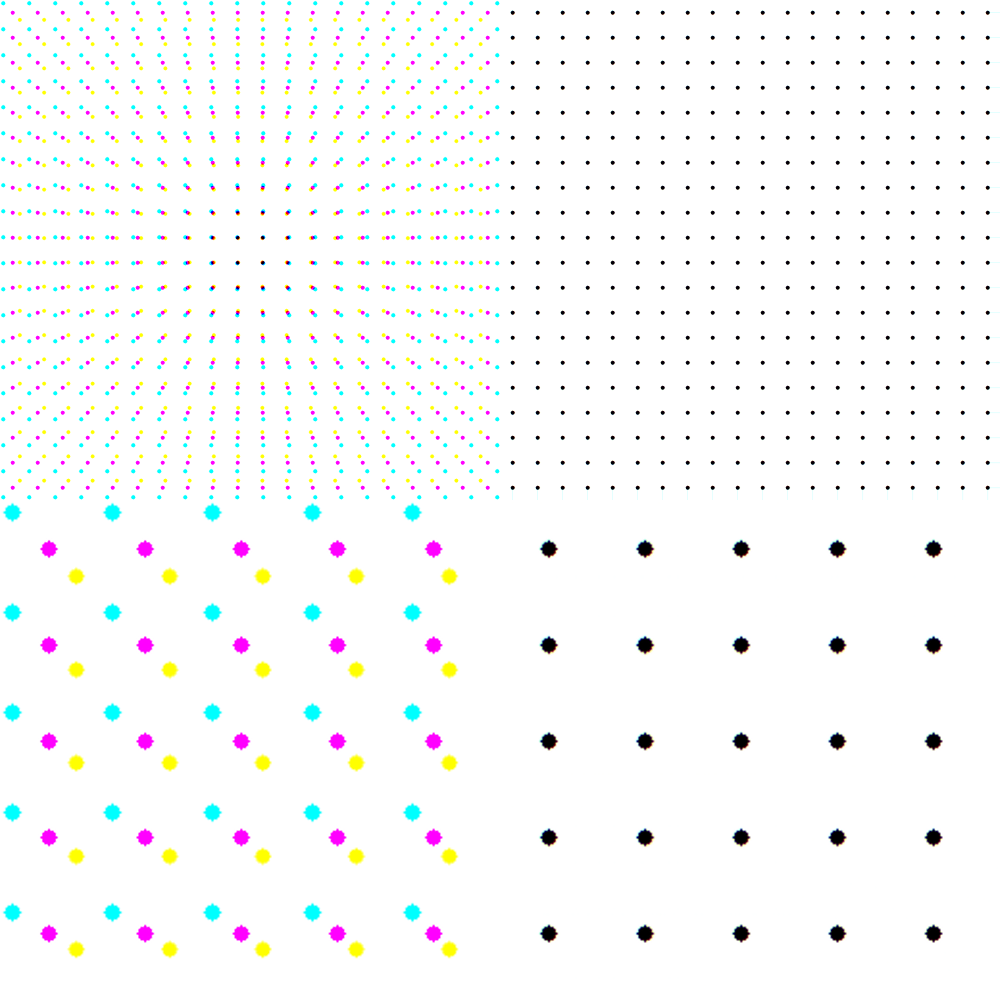
\includegraphics[width=0.52\textwidth]{figures/fig_target.png}
\caption{Синтетическая точечная мишень $1000\times1000$ с известной
аберрацией ($k_R = 0{,}04$, $k_B = -0{,}03$): сверху --- до и после
коррекции, снизу --- угол мишени}
\label{fig:target}
\end{figure}

Третье проявление --- остаточная цветная кайма. У контрастной границы канал
с большей расфокусировкой формирует размытую цветную «юбку», которая не
сводится к сдвигу канала; её источники --- продольная аберрация,
дифракция, демозаикинг и внутрикамерное повышение резкости. Кайма
локализована у границ, а потеря резкости глобальна, по этой причине в работе это
разные стадии конвейера.

\subsection{Математическая модель искажения}

Координаты нормируются на половину диагонали кадра: $u=(x-c_x)/s$,
$v=(y-c_y)/s$, $\rho^2=u^2+v^2$, $s=\tfrac12\sqrt{w^2+h^2}$, где $w$ и $h$
--- ширина и высота. Поле смещений канала $c \in \{B,R\}$ относительно
зелёного описывается радиально-аффинным полиномом
\begin{equation}
d_{x,c}=t_{x,c}+\bigl(a_{x,c}+b_{x,c}\rho^2\bigr)u, \qquad
d_{y,c}=t_{y,c}+\bigl(a_{y,c}+b_{y,c}\rho^2\bigr)v,
\label{eq:field}
\end{equation}
где $t$ --- постоянный сдвиг, $a$ и $b$ --- линейные и кубические
радиальные коэффициенты; при $b=0$ модель сводится к аффинной.
Калибровочный режим использует скалярную радиальную модель
\begin{equation}
d(r)=c_1 r+c_2 r^2+c_3 r^3,
\label{eq:poly}
\end{equation}
коэффициенты которой находятся методом наименьших квадратов (МНК)~[4, 5].

Локальный сдвиг вдоль нормали к границе измеряется как аргумент максимума
нормированной взаимной корреляции (NCC) профилей опорного и
измеряемого каналов:~[6]
\begin{equation}
\rho(s)=\frac{\sum_t (g(t)-\bar g)\,(c(t+s)-\bar c_s)}
{\sqrt{\sum_t (g(t)-\bar g)^2\sum_t (c(t+s)-\bar c_s)^2}},
\label{eq:ncc}
\end{equation}
а максимум уточняется до субпиксельной точности параболической
интерполяцией трёх отсчётов:
\begin{equation}
\hat s=s^{*}+\frac{1}{2}\cdot\frac{y_{-}-y_{+}}{y_{-}-2M+y_{+}},
\label{eq:subpixel}
\end{equation}
где $M$ --- значение корреляции в максимуме $s^{*}$, $y_{\pm}$ ---
значения в соседних отсчётах. Коэффициенты \eqref{eq:field} находятся
робастным МНК с перевзвешиванием по функции Тьюки и гребневой
регуляризацией: это нейтрализует выбросы и нестабильные решения на кадрах с
малым числом надёжных границ.

Кайма описывается моделью линейного смешения цветов вдоль нормали к
границе. Пусть $C_{\text{dark}}$ и $C_{\text{bright}}$ --- значения канала
на тёмной и светлой сторонах, полученные сдвигом на $\pm p_s$ вдоль
градиента поля расстояний до яркой области. Прозрачность перехода,
ожидаемое значение канала и отклонение равны
\begin{equation}
\begin{aligned}
\alpha&=\operatorname{clip}\!\left(\frac{G-G_{\text{dark}}}
{G_{\text{bright}}-G_{\text{dark}}},0,1\right),\\
C_{\text{exp}}&=C_{\text{dark}}+(C_{\text{bright}}-C_{\text{dark}})\alpha,
\qquad d_C=C-C_{\text{exp}},
\end{aligned}
\label{eq:fringe}
\end{equation}
а коррекция вводится с маской уверенности $m\in[0,1]$ и коридором
допустимых значений $[h^{-};h^{+}]$, расширенным на восемь уровней:
\begin{equation}
\Delta_C=m\cdot\operatorname{clip}\!\left(d_C,\;C-h^{+},\;C-h^{-}\right).
\label{eq:correction}
\end{equation}
Ограничение \eqref{eq:correction} удерживает результат в пределах диапазона
цветов сторон границы.

Продольная составляющая описывается моделью наблюдения
$C=h_C\otimes F+n$, где $F$ --- сфокусированный сигнал, $n$ --- шум, а ядро
--- гауссова функция с передаточной функцией
\begin{equation}
h_C(x,y)=\frac{1}{2\pi\sigma_C^2}\exp\!\left(-\frac{x^2+y^2}
{2\sigma_C^2}\right),\qquad
K_C(\omega)=\exp\!\left(-\frac{\sigma_C^2\omega^2}{2}\right),
\label{eq:axial_kernel}
\end{equation}
$\sigma_G=0$ для опорного зелёного канала. Обращение $K_C$ некорректно:
на высоких частотах оно неограниченно усиливает шум~[1, 7], поэтому в работе
восстановление выполнено с помощью итеративного алгоритма
Ричардсона--Люси~[8, 9]
\begin{equation}
u_{k+1}=u_k\cdot\left(h_C^{*}\otimes\frac{C}{h_C\otimes u_k}\right),
\label{eq:rl}
\end{equation}
где звёздочка --- сопряжение, деление поэлементно.

\subsection{Обзор существующих решений}

Сравнение существующих средств и разрабатываемого ПО приведено в
таблице~\ref{tab:compare}.

\begin{table}[H]
\caption{Обзор существующих средств коррекции хроматических аберраций}
\label{tab:compare}
\small
\begin{tabular}{|p{3.4cm}|p{3.8cm}|p{7.6cm}|}
\hline
Средство & Режим коррекции & Модель и особенности \\
\hline
Adobe Lightroom & профиль или ручная правка & попиксельные ползунки, интерактивная работа \\
\hline
OpenCV & по кадру мишени & полином высокой степени, МНК~[10] \\
\hline
Hugin (fulla) & по контрольным точкам & полином по радиусу \\
\hline
RawTherapee и др. & по порогу насыщенности & обесцвечивание кромок без модели смешения \\
\hline
Разрабатываемое ПО & калибровка и слепой режим & поле \eqref{eq:field}, ядро \eqref{eq:axial_kernel}, смешение \eqref{eq:fringe} \\
\hline
\end{tabular}
\end{table}

Редакторы предлагают применять профили объективов либо ручную правку и в основном рассчитаны на
интерактивную работу. OpenCV предоставляет коррекцию по кадру мишени с
полиномиальной моделью~[10]: данное решение универсально, но требует калибровочного
кадра и не имеет слепого режима. Слепая оценка поперечной аберрации по
одному снимку известна из работ~[11, 12], однако стадия подавления
остаточной каймы в них не выделена. Инструменты дефринджа работают по порогу
насыщенности и не отличают цвет объекта от цвета каймы, из-за чего
обесцвечивают легитимные насыщенные объекты. Разрабатываемое ПО объединяет
калибровочный и слепой режимы со стадиями компенсации продольной аберрации и
подавления каймы по модели смешения.

\subsection{Выбор средств реализации}

Вычислительное ядро реализовано на Python с библиотеками NumPy~[13] и
OpenCV~[10]: они дают быстрые свёртки, морфологию, карты расстояний и
преобразования Фурье, достаточные для всех стадий. Интерфейс построен на
стандартном Tk, тесты --- на pytest, что избавляет от внешних зависимостей.
Критичные участки (спектральные оценки, деконволюция) векторизованы.

\section{Конструкторская часть}

\subsection{Требования к программному обеспечению}

ПО должно:
\begin{enumerate}
\item брать на вход цветные изображения BGR в формате uint8 и не изменять их, если искажения нет;
\item выполнять слепую коррекцию без калибровочного кадра и калибровочную по
кадру точечной мишени;
\item подавлять остаточную кайму, не обесцвечивая естественные насыщенные
объекты;
\item опционально компенсировать продольную аберрацию;
\item сохранять результат на диск до показа и вести журнал;
\item работать из командной строки пакетно.
\end{enumerate}

\subsection{Архитектура программной системы}

Система разделена на вычислительное ядро (пакет \texttt{achrom}) и уровень
приложения (\texttt{app.py}); ядро не зависит от интерфейса. Единая точка
входа --- \texttt{process\_frame} из \texttt{pipeline.py}: функция проводит
кадр через конвейер «геометрическая регистрация, компенсация продольной аберрации,
подавление каймы» (рисунок~\ref{fig:arch}).

\begin{figure}[H]
\centering
\resizebox{0.95\linewidth}{!}{%
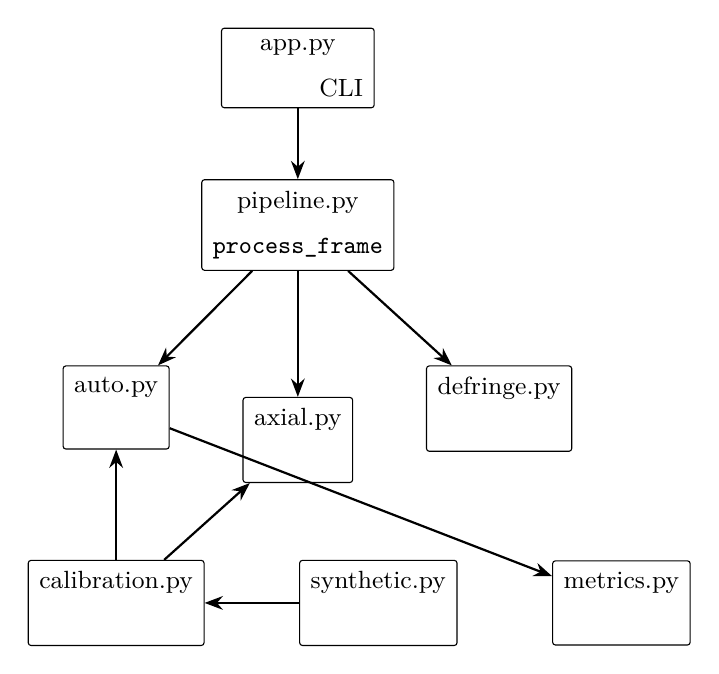
\begin{tikzpicture}[
  node distance=9mm and 12mm,
  box/.style={draw,rounded corners=1pt,align=center,inner sep=4pt,
              minimum height=9mm,font=\small},
  arr/.style={-{Stealth[]},thick}]
\node[box] (app) {app.py\\интерфейс и CLI};
\node[box,below=of app] (pipe) {pipeline.py\\\texttt{process\_frame}};
\node[box,below left=12mm and 4mm of pipe] (auto) {auto.py\\геометрия};
\node[box,below right=12mm and 4mm of pipe] (defr) {defringe.py\\кайма};
\node[box,below=16mm of pipe] (axial) {axial.py\\продольная};
\node[box,below=14mm of auto] (calib) {calibration.py\\калибровка};
\node[box,right=of calib] (synth) {synthetic.py\\генератор мишени};
\node[box,right=of synth] (metrics) {metrics.py\\остаток};
\draw[arr] (app) -- (pipe);
\draw[arr] (pipe) -- (auto);
\draw[arr] (pipe) -- (defr);
\draw[arr] (pipe) -- (axial);
\draw[arr] (synth) -- (calib);
\draw[arr] (calib) -- (auto);
\draw[arr] (calib) -- (axial);
\draw[arr] (auto) -- (metrics);
\end{tikzpicture}}
\caption{Архитектура программной системы}
\label{fig:arch}
\end{figure}

\texttt{auto.py} осуществляет слепую оценку поля, робастную подгонку
\eqref{eq:field} и обратный варп; \texttt{defringe.py} подавляет кайму по
\eqref{eq:fringe}--\eqref{eq:correction}; \texttt{axial.py} измеряет ядра,
определяет расфокусировку и деконволюцирует; \texttt{calibration.py}
калибрует по точечному кадру~[5, 14]; \texttt{synthetic.py} и
\texttt{metrics.py} дают генератор мишени и метрики остатка.

\subsection{Геометрическая регистрация каналов}

Опорные точки --- пиксели с максимальным откликом градиента в зелёном
канале, равномерно распределённые по ячейкам сетки. Профили каналов вдоль нормали к границе сравниваются по
\eqref{eq:ncc} с субпиксельным уточнением \eqref{eq:subpixel}. Измерению
задается вес по контрасту границы, малоконтрастные точки отсеиваются.

Коэффициенты \eqref{eq:field} находятся итеративно перевзвешенным МНК
(IRLS): на каждой из 12 итераций
решается гребневая задача МНК с весами Тьюки $w_i=(1-(|r_i|/(4{,}685\,\hat
\sigma))^2)^2$ для невязок меньше $4{,}685\hat\sigma$, где $\hat\sigma$ ---
робастная оценка масштаба по MAD. Кубический член стабилизируется
ограничением $\rho^2$ сверху 97-м процентилем по опорным точкам.

Накопленное поле смещений проецируется на полный кадр бикубическим варпом:
смещения оцениваются на сетке с шагом 16~пикселей, а карта достраивается
билинейно. Сетка равномерна и выходит за край кадра, так что карта
тождественна нулевому смещению на всей области, включая последнюю неполную
ячейку.

Коррекция применяется итеративно (до пяти шагов), причем каждый шаг проверяется
повторным измерением остатка на тех же границах: модель принимается, если
оценка улучшилась не менее чем на 1{,}5~\% и 95-й процентиль не вырос более
чем на 10~\%; при слабом шаге амплитуда уменьшается вдвое-вчетверо. Шаг
меньше 0{,}25~пикс или поле больше 18~пикс останавливает итерации.

\subsection{Калибровка объектива по точечному кадру}

Калибровка ищет диски мишени в каждом канале по центрам масс окрестности
(годится и для тёмных точек на светлом фоне, и наоборот --- знак контраста
учитывается), сопоставляет точки между каналами и вычисляет радиальные
смещения. Коэффициенты \eqref{eq:poly} находятся МНК. На синтетическом кадре
с заведомо известными коэффициентами среднее расхождение каналов
уменьшилось с 12{,}71 до 0{,}00~пикс, максимальное --- с 25{,}46 до
0{,}00~пикс.

Коэффициенты зависят от размера кадра мишени: при другом масштабе их нужно
перенормировать, иначе кубический полином уйдёт в нефизичную область. Поэтому интерфейс ориентирован на слепой режим, а калибровочный
шов сохранён в библиотеке и покрыт тестами.

\subsection{Подавление остаточной цветной каймы}

Основной проход оценивает по маскам чистых «светлых» и «тёмных» пикселей
цветовые отношения $C/G$ фона и переднего плана нормированной свёрткой,
строит ожидаемое значение по \eqref{eq:fringe} и корректирует отклонение по
\eqref{eq:correction} в переходной зоне $0{,}02<\alpha<0{,}95$ при
$|d_C|>18$. Синий канал обрабатывается по избытку синего, красный --- по
дефициту красного на пурпурной кромке. Гейт пурпура отключает коррекцию,
если избыток красного сопоставим с избытком синего: это цвет объекта, а не
кайма.

Проход для маджента-каёмок строит доказательство каймы по глубокой пробе
вдоль градиента поля расстояний и эрозионному минимуму обоих каналов, а
также по признаку тонкой полосы; естественный пурпур отличается от каймы
малым отношением сырых разностей $B-G$ и $R-G$. Профильный проход работает
на цветных фонах: нормаль берётся к градиенту поля расстояний до яркой
области, поэтому фон не обязан быть нейтральным. Если нейтрально-ярких
пикселей меньше ста, маска переднего плана строится по верхнему децилю
яркости.

Остаток измеряется по исправленному изображению, сигнатура каймы --- по
исходному, что исключает двойную коррекцию. Маска $m<1$ делает коррекцию
частичной, из-за чего повторные прогоны сходятся монотонно.

\subsection{Компенсация продольной аберрации}

\textbf{Измерение ядра по мишени.} Точка мишени --- приближение
дельта-импульса, поэтому отношение спектров канала и зелёного канала в
окне $21\times21$ пиксель оценивает $K_C$. Спектр каждого окна
центрируется по субпиксельному положению точки: фазовый множитель
$\exp(2\pi i(\omega_x(c_x-x)+\omega_y(c_y-y)))$ снимает линейный набег фазы,
вызванный её смещением от центра окна. Взвешенный МНК (веса --- энергия
спектра) по зависимости $\ln K_C=-\sigma_C^2\omega^2/2$ в полосе, где
отношение достоверно, даёт $\sigma_C$; итоговое ядро --- аналитический
гауссиан. Ядра заданы в пикселях кадра мишени.

\textbf{Слепая оценка.} $\sigma_C$ подбирается по самому снимку: из зелёного канала
синтезируются гауссово размытые копии, и выбирается $\sigma$, минимизирующий
невязку с каналом $C$ после подгонки масштаба. Оценка ведётся на фрагменте
$512\times512$ в родном разрешении; фрагмент выбирается по максимальной
дисперсии лапласиана, то есть по наиболее богатой текстуре кадра. Уменьшать копию
перед оценкой нельзя: это сжимает $\sigma$ ниже шага перебора и
занижает расфокусировку на крупных кадрах. Верхняя граница поиска ---
1{,}2~пикс: цветовая субдискретизация JPEG ($4{:}2{:}0$) сама вносит
размытие порядка пикселя.

\textbf{Деконволюция.} Восстановление выполняется по \eqref{eq:rl} в
частотной области над зеркально расширенным кадром; результат каждой
итерации ограничивается диапазоном $[0;255]$. Применяется 12 итераций для
кадров до 2~Мпикс и 6 для более крупных. При $\hat\sigma_C<0{,}2$~пикс
канал считается сфокусированным и не изменяется.

\subsection{Графический интерфейс и пакетная обработка}

Интерфейс на Tk показывает снимок, зум и результат «до/после». Обработка
идёт в фоновом потоке, результат передаётся главному потоку через очередь и
поллинг: Tk не потокобезопасен, а вызовы \texttt{after} из рабочего потока
на системном Tcl/Tk macOS молча завершают процесс. Изображения результата
пишутся в PNG до показа, поэтому закрытие окна во время обработки не теряет
данные. Все действия кнопок обёрнуты обработчиком, который пишет трейсбек в
\texttt{app.log} и показывает сообщение.

Пакетный режим принимает файлы и каталоги, поддерживает флаг
\texttt{--axial} и калибровочный ключ \texttt{--axial-cal}; имена результатов
сохраняют исходное имя файла с точками. В журнал пишутся размеры кадра,
решение каждой стадии и тайминги.

\section{Технологическая часть}

\subsection{Технологический стек}

Python 3.9, NumPy~[13], OpenCV~[10], Pillow (загрузка снимков), Tk
(интерфейс), pytest (тесты). Новые зависимости не вводились: все стадии
покрываются стандартным набором.

\subsection{Организация исходного кода}

Пакет \texttt{achrom} содержит модули геометрии, каймы, продольной
аберрации, калибровки, метрик, альтернативных оценок и генератора мишени;
\texttt{app.py} --- интерфейс и CLI. Правило одно: ядро не импортирует
интерфейс. Фрагменты кода вынесены в приложения А--Г.

\subsection{Модульное тестирование}

Тесты написаны по схеме red--green: сначала падающий тест на публичный шов,
затем минимальный код. Ожидаемые значения берутся из независимой истины ---
известных коэффициентов генератора мишени или ручного расчёта --- и не
пересчитываются тем же способом, что и реализация. Проверяются обнаружение
точек, субпиксельная точность, снятие известной латеральной аберрации,
восстановление известной расфокусировки, подавление каймы без обесцвечивания
фона, идемпотентность и отказы на некорректном входе. Всего 60 тестов, все
проходят.

\section{Аналитическая часть}

\subsection{Тестовые данные}

Открытых микрофотографий с известными параметрами аберрации нет, так что
корпус (размеры в мегапикселях, Мпикс) собран из снимков с похожим характером искажений: макросъёмка,
объективы без хроматической коррекции, игрушечная оптика, кадры с цветными
каёмками (таблица~\ref{tab:data}). Кадр \texttt{real\_blende8.jpg} снят
камерой с внутрикамерной коррекцией и служит контролем ложных срабатываний
геометрии; \texttt{mytestcheck.png} и \texttt{holga\_tatra.jpg} содержат
большие области естественного цвета и контролируют его сохранение.

\begin{table}[H]
\caption{Характеристики тестовых изображений}
\label{tab:data}
\small
\begin{tabular}{|p{3.4cm}|p{6.2cm}|p{2.5cm}|p{2.3cm}|}
\hline
Файл & Содержание & Разрешение & Пикселей \\
\hline
another.png & синее небо, ветки, синяя и жёлтая кайма & 705$\times$465 & 0,33~Мпикс \\
\hline
blur.png & дифракционный объектив, боке & 886$\times$1585 & 1,40~Мпикс \\
\hline
detail\_ca.jpg & дуга, широкая синяя кайма & 2592$\times$2592 & 6,72~Мпикс \\
\hline
flower.jpeg & пурпурные лепестки, малый кадр & 300$\times$199 & 0,06~Мпикс \\
\hline
holga\_tatra.jpg & игрушечная оптика, синее небо & 3840$\times$2566 & 9,85~Мпикс \\
\hline
lens\_ca.jpg & радужный блик объектива & 2462$\times$2532 & 6,23~Мпикс \\
\hline
mytestcheck.png & пурпурный фон, частицы & 5184$\times$2912 & 15,10~Мпикс \\
\hline
pigeon.jpg & тонированный кадр & 250$\times$454 & 0,11~Мпикс \\
\hline
real\_blende8.jpg & внутрикамерная коррекция & 2000$\times$1328 & 2,66~Мпикс \\
\hline
tree.jpg & ветки на фоне неба & 720$\times$482 & 0,35~Мпикс \\
\hline
tree2.jpg & ветки на фоне неба & 1200$\times$639 & 0,77~Мпикс \\
\hline
\end{tabular}
\end{table}

\subsection{Результаты геометрической регистрации}

Геометрическая стадия выполнена для каждого кадра; остаток измерен как
медиана модуля сдвига на опорных границах (таблица~\ref{tab:geometry}).

\begin{table}[H]
\caption{Результаты геометрической регистрации каналов}
\label{tab:geometry}
\small
\begin{tabular}{|p{3.0cm}|p{1.8cm}|p{2.4cm}|p{3.0cm}|p{3.0cm}|}
\hline
Изображение & Итераций & Макс.\ сдвиг B / R, пикс & Остаток B до / после, пикс & Остаток R до / после, пикс \\
\hline
another.png & 1 & 0,00 / 1,34 & 0,72 / 0,72 & 0,62 / 0,48 \\
\hline
blur.png & 0 & 0,00 / 0,00 & 0,11 / 0,11 & 0,12 / 0,12 \\
\hline
detail\_ca.jpg & 0 & 0,00 / 0,00 & 0,01 / 0,01 & 0,01 / 0,01 \\
\hline
flower.jpeg & 1 & 2,53 / 1,53 & 1,80 / 0,10 & 1,25 / 0,34 \\
\hline
holga\_tatra.jpg & 1 & 0,84 / 1,79 & 0,15 / 0,10 & 0,19 / 0,12 \\
\hline
lens\_ca.jpg & 1 & 0,30 / 0,00 & 0,10 / 0,09 & 0,08 / 0,08 \\
\hline
mytestcheck.png & 1 & 7,50 / 1,54 & 0,86 / 0,72 & 0,82 / 0,75 \\
\hline
pigeon.jpg & 0 & 0,00 / 0,00 & 0,05 / 0,05 & 0,01 / 0,01 \\
\hline
real\_blende8.jpg & 0 & 0,00 / 0,00 & 0,42 / 0,42 & 0,26 / 0,26 \\
\hline
tree.jpg & 0 & 0,00 / 0,00 & 0,02 / 0,02 & 0,04 / 0,04 \\
\hline
tree2.jpg & 0 & 0,00 / 0,00 & 0,06 / 0,06 & 0,05 / 0,05 \\
\hline
\end{tabular}
\end{table}

Наибольшее смещение --- у \texttt{mytestcheck.png} (синий канал 7,50~пикс к
краю поля) и у малого \texttt{flower.jpeg} (2,53~пикс). На остальных кадрах
поле субпиксельное: коррекция либо не применяется, либо ограничивается одной
итерацией. Контрольные кадры (\texttt{real\_blende8}, \texttt{pigeon},
\texttt{tree}, \texttt{tree2}) не изменяются: измеренный остаток ниже порога
0{,}25~пикс. У кадров с сильной каймой (\texttt{lens\_ca},
\texttt{detail\_ca}) медианное смещение мало, так как их искажение ---
размытая цветная «юбка», а не сдвиг; это подтверждает необходимость
двухкомпонентной модели.

\subsection{Результаты подавления остаточной каймы}

В таблице~\ref{tab:defringe} приведены число исправленных пикселей, их доля
от кадра и среднее абсолютное изменение каналов.

\begin{table}[H]
\caption{Результаты подавления остаточной цветной каймы}
\label{tab:defringe}
\small
\begin{tabular}{|p{3.3cm}|p{2.3cm}|p{1.9cm}|p{2.6cm}|p{2.6cm}|}
\hline
Изображение & Исправлено, пикс & Доля кадра, \% & Среднее $|\Delta B|$ & Среднее $|\Delta R|$ \\
\hline
another.png & 28\,298 & 8,63 & 2,48 & 0,92 \\
\hline
blur.png & 66\,851 & 4,76 & 1,28 & 0,98 \\
\hline
detail\_ca.jpg & 201\,371 & 3,00 & 1,49 & 0,67 \\
\hline
flower.jpeg & 2\,080 & 3,48 & 0,51 & 0,94 \\
\hline
holga\_tatra.jpg & 114\,176 & 1,16 & 0,12 & 0,06 \\
\hline
lens\_ca.jpg & 341\,362 & 5,48 & 2,35 & 1,14 \\
\hline
mytestcheck.png & 16\,301 & 0,11 & 0,01 & 0,01 \\
\hline
pigeon.jpg & 2\,309 & 2,03 & 0,13 & 0,06 \\
\hline
real\_blende8.jpg & 19\,929 & 0,75 & 0,20 & 0,04 \\
\hline
tree.jpg & 10\,650 & 3,07 & 0,76 & 1,01 \\
\hline
tree2.jpg & 122\,896 & 16,03 & 10,69 & 7,29 \\
\hline
\end{tabular}
\end{table}

На нейтральных фонах дополнительно измерено число пикселей с выраженным
цветным избытком: сине-голубая кайма --- условие $B-G\ge20$ и
$B-R\ge20$, маджента-кайма --- $R-G\ge15$ и $B-G\ge15$. Сине-голубых
пикселей у \texttt{detail\_ca.jpg} стало 3\,704 против 129\,279 (уменьшение
на 97,1~\%); у \texttt{lens\_ca.jpg} --- 14\,489 против 216\,433
(на 93,3~\%). Маджента-пикселей у \texttt{tree2.jpg} стало 18\,708 против
107\,431 (на 82,6~\%); у \texttt{tree.jpg} --- 3\,347 против 7\,610
(на 56,0~\%). Естественный фон при этом остаётся прежним: у
\texttt{mytestcheck.png} исправлено 0,11~\% пикселей, пурпурный фон и жёлтые
объекты сохраняются; у \texttt{holga\_tatra.jpg} исправлено 1,16~\%,
открытое небо остаётся. На цветных фонах счётчик цветных пикселей не служит
критерием качества, поскольку фон сам удовлетворяет порогу.

Фрагменты «до/после» приведены на рисунках~\ref{fig:lens}, \ref{fig:tree2},
\ref{fig:flower} и \ref{fig:detail}.

\begin{figure}[H]
\centering
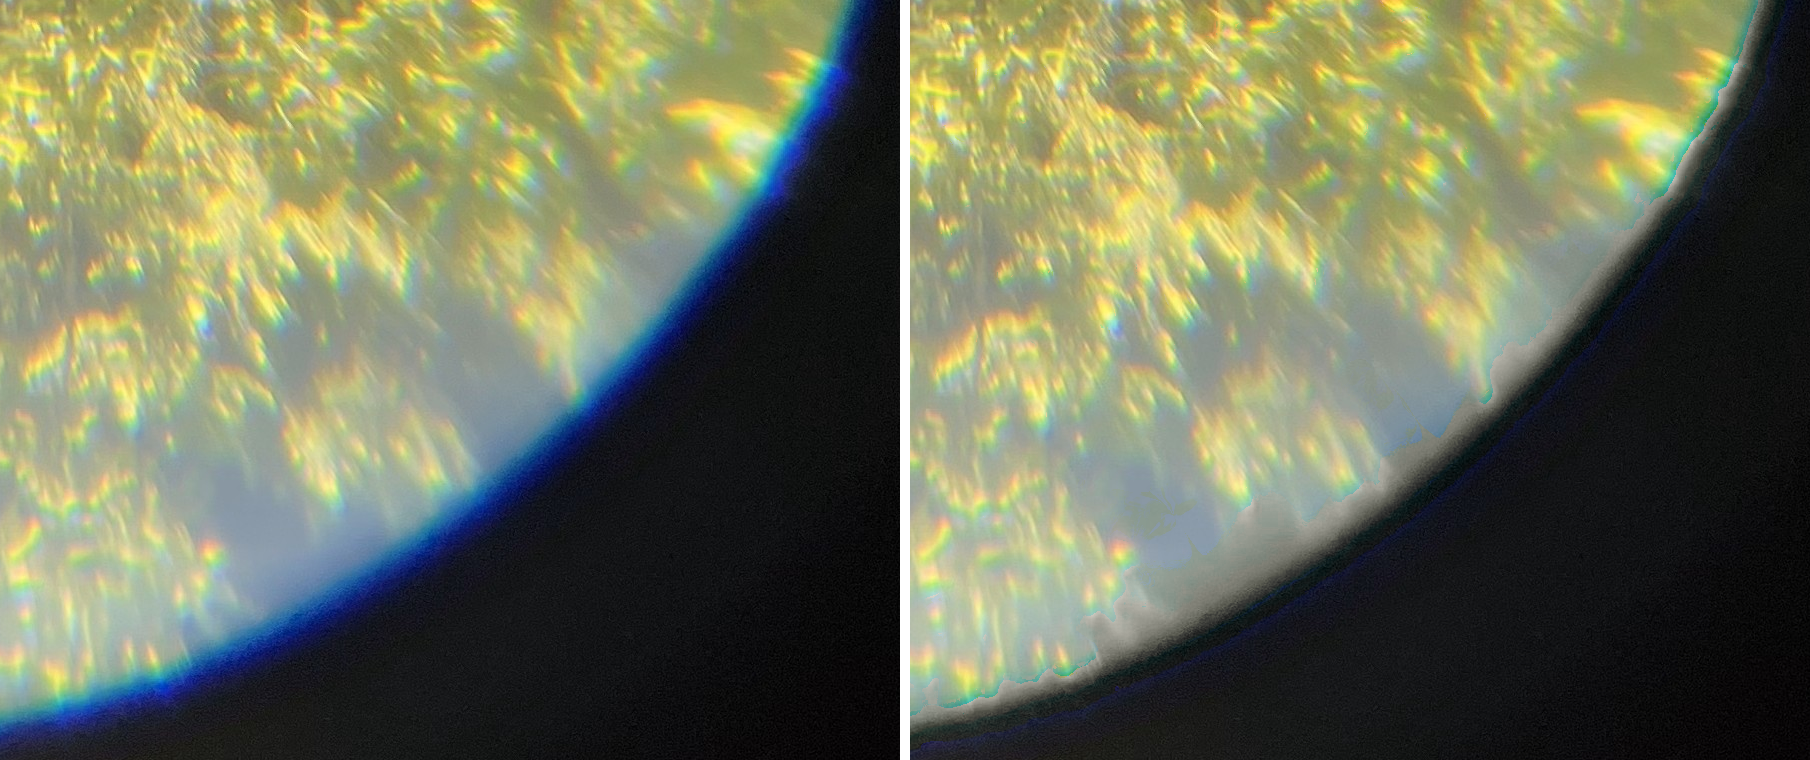
\includegraphics[width=0.95\textwidth]{figures/fig_lens.png}
\caption{Устранение сильной цветной каймы (\texttt{lens\_ca.jpg}):
слева --- до, справа --- после}
\label{fig:lens}
\end{figure}

\begin{figure}[H]
\centering
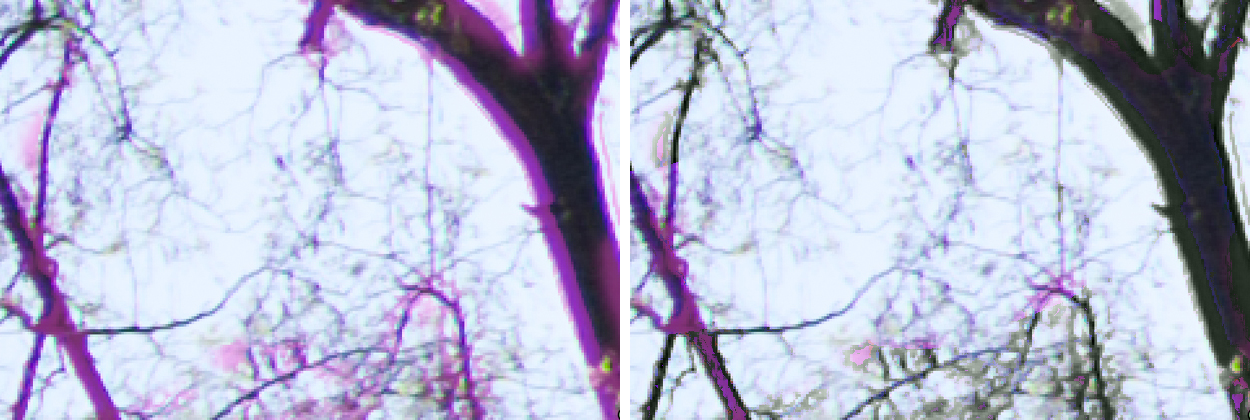
\includegraphics[width=0.95\textwidth]{figures/fig_tree2.png}
\caption{Удаление маджента-каёмок вдоль веток (\texttt{tree2.jpg}):
слева --- до, справа --- после}
\label{fig:tree2}
\end{figure}

\begin{figure}[H]
\centering
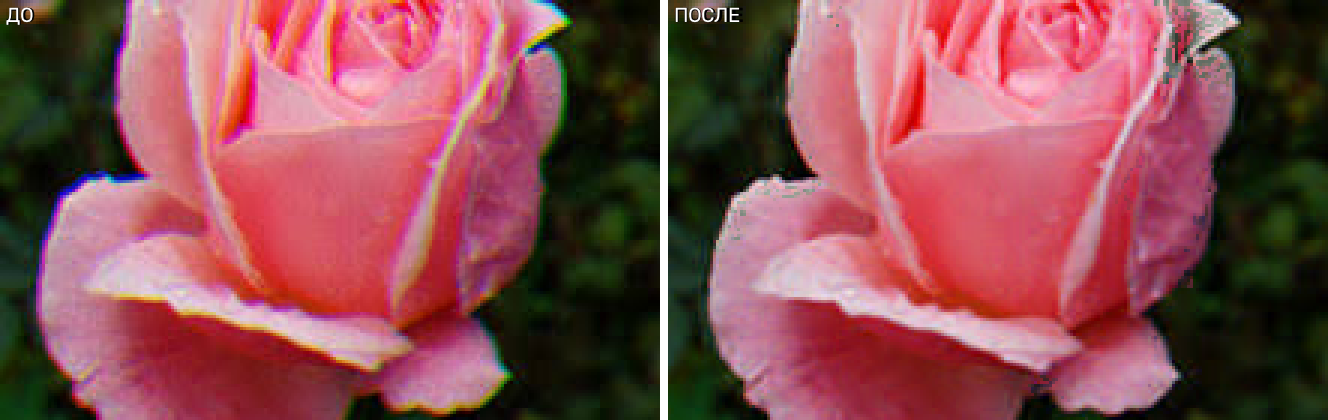
\includegraphics[width=0.85\textwidth]{figures/fig_flower.png}
\caption{Фиолетовые ореолы у лепестков (\texttt{flower.jpeg}):
слева --- до, справа --- после}
\label{fig:flower}
\end{figure}

\begin{figure}[H]
\centering
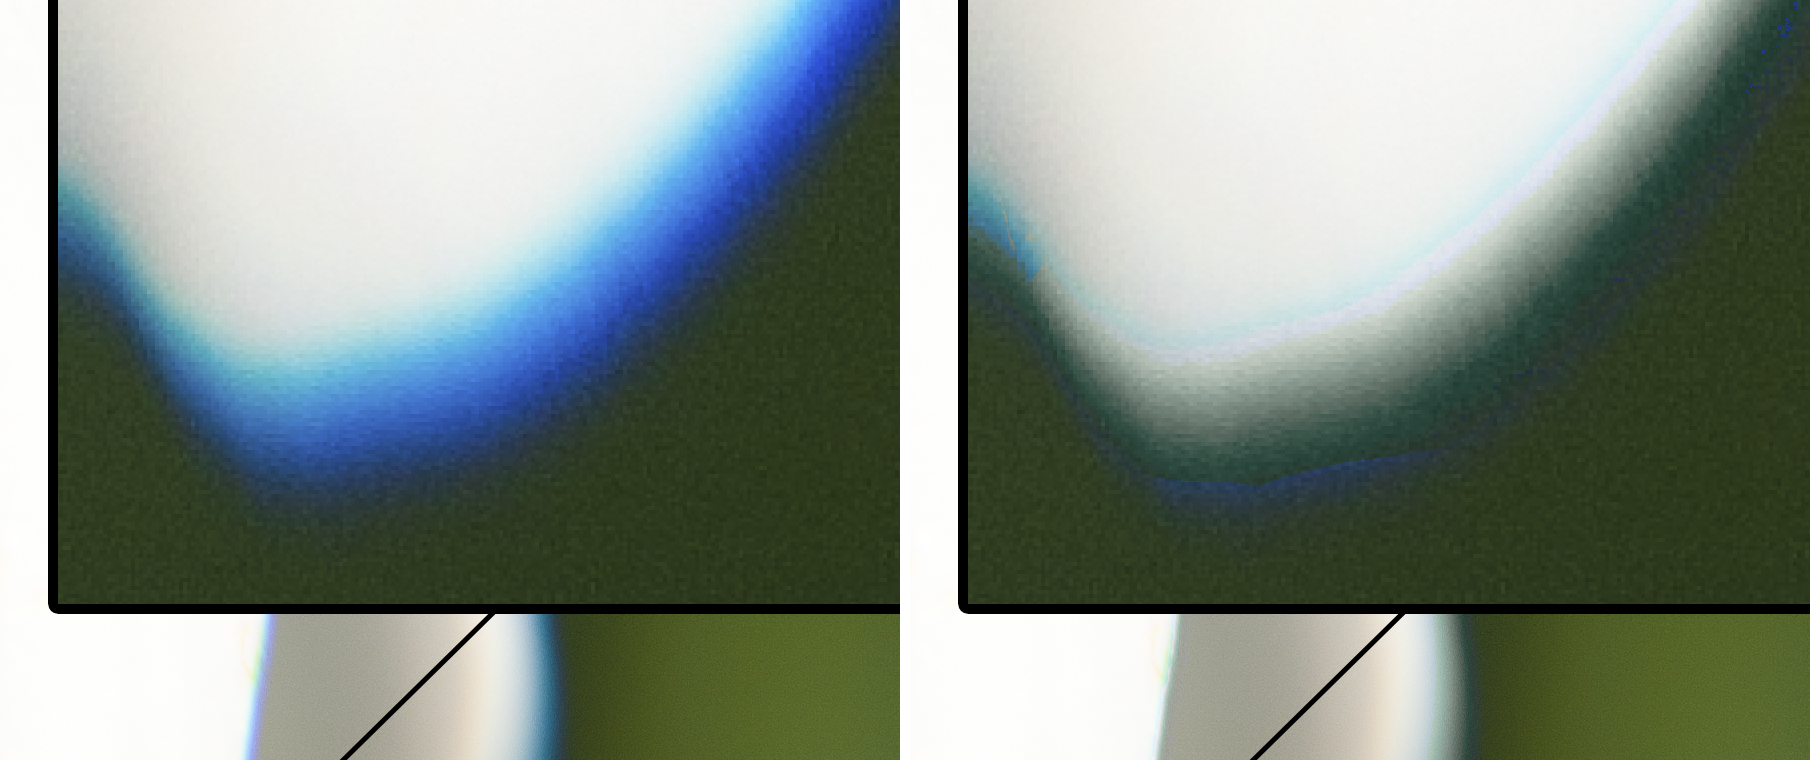
\includegraphics[width=0.85\textwidth]{figures/fig_detail.png}
\caption{Сине-голубая кайма на контуре (\texttt{detail\_ca.jpg}):
слева --- до, справа --- после}
\label{fig:detail}
\end{figure}

\subsection{Результаты компенсации продольной аберрации}

Точность измерения ядер мы проверили на синтетических кадрах, где гауссова
расфокусировка известна заранее (таблица~\ref{tab:axial_syn}). При
$\sigma\ge0{,}6$~пикс измеренное ядро восстанавливает истинное с точностью до
0{,}1~пикс: при $\sigma_R=2{,}5$ оценка равна 2{,}50. Субпиксельная
расфокусировка ($\sigma\le0{,}4$) занижается до нуля: на высоких частотах спектр точки
уже не отличить от шума квантования, поэтому коррекция просто не включается,
а кадр остаётся нетронутым. Корреляция восстановленного канала с
эталоном возрастает во всех случаях, где коррекция выполнялась.

\begin{table}[H]
\caption{Восстановление известной расфокусировки на синтетике}
\label{tab:axial_syn}
\small
\begin{tabular}{|p{1.5cm}|p{1.5cm}|p{1.5cm}|p{1.5cm}|p{3.1cm}|p{3.1cm}|}
\hline
Задано $\sigma_R$ & Задано $\sigma_B$ & Оценка $\hat\sigma_R$ & Оценка $\hat\sigma_B$ & Корреляция R, до / после & Корреляция B, до / после \\
\hline
0,6 & 0,4 & 0,51 & 0,01 & 0,977 / 0,994 & 0,998 / 0,998 \\
\hline
1,0 & 0,6 & 1,00 & 0,51 & 0,938 / 0,959 & 0,977 / 0,994 \\
\hline
1,5 & 1,0 & 1,49 & 1,00 & 0,903 / 0,932 & 0,938 / 0,959 \\
\hline
2,5 & 1,5 & 2,50 & 1,49 & 0,835 / 0,879 & 0,903 / 0,932 \\
\hline
0,0 & 0,8 & 0,00 & 0,77 & 1,000 / 1,000 & 0,955 / 0,976 \\
\hline
0,4 & 0,0 & 0,01 & 0,00 & 0,998 / 0,998 & 1,000 / 1,000 \\
\hline
\end{tabular}
\end{table}

На реальных кадрах стадия проверена в слепом режиме
(таблица~\ref{tab:axial_real}); резкость канала --- отношение дисперсий
лапласиана данного канала и зелёного. На кадрах с заметной расфокусировкой
резкость каналов относительно зелёного возрастает в 1,2--5,2~раза при росте
шума в плоских областях не более чем в 1,6~раза.

\begin{table}[H]
\caption{Компенсация продольной аберрации на реальных кадрах (слепой
режим)}
\label{tab:axial_real}
\small
\begin{tabular}{|p{3.0cm}|p{2.4cm}|p{2.7cm}|p{2.7cm}|p{1.7cm}|}
\hline
Изображение & $\hat\sigma_B$ / $\hat\sigma_R$, пикс & Резкость B/G, до / после & Резкость R/G, до / после & Время, мс \\
\hline
another.png & 1,20 / 0,50 & 1,10 / 3,60 & 1,12 / 1,95 & 601 \\
\hline
blur.png & 1,20 / 1,20 & 0,99 / 1,69 & 0,91 / 1,48 & 3\,741 \\
\hline
detail\_ca.jpg & 0,50 / 0,40 & 0,93 / 2,09 & 0,96 / 1,29 & 5\,397 \\
\hline
flower.jpeg & 0,90 / 1,20 & 1,40 / 5,17 & 0,98 / 2,99 & 92 \\
\hline
holga\_tatra.jpg & 0,60 / 1,20 & 1,03 / 2,52 & 1,03 / 1,60 & 10\,599 \\
\hline
lens\_ca.jpg & 0,00 / 0,40 & 1,05 / 1,02 & 1,02 / 1,36 & 4\,784 \\
\hline
mytestcheck.png & 1,20 / 1,20 & 0,26 / 0,71 & 0,32 / 0,81 & 26\,450 \\
\hline
pigeon.jpg & 0,40 / 0,30 & 0,95 / 1,25 & 0,99 / 1,01 & 139 \\
\hline
real\_blende8.jpg & 0,50 / 0,00 & 0,98 / 2,07 & 1,04 / 1,04 & 2\,458 \\
\hline
tree.jpg & 0,40 / 0,50 & 0,99 / 1,22 & 0,98 / 1,77 & 341 \\
\hline
tree2.jpg & 0,00 / 0,00 & 0,87 / 0,87 & 0,91 / 0,91 & 361 \\
\hline
\end{tabular}
\end{table}

Слепая оценка в родном разрешении чувствительна к хроматической
субдискретизации JPEG: почти у всех кадров $\hat\sigma_B\ge0{,}4$, а у
\texttt{mytestcheck.png} и \texttt{holga\_tatra.jpg} оценка упирается в
потолок 1{,}2~пикс. Коррекция включается при $\hat\sigma\ge0{,}2$, отсюда
«нулевых» кадров почти нет; единственный неизменённый кадр ---
\texttt{tree2.jpg} ($\hat\sigma_B=\hat\sigma_R=0$). Изменение кадра при
$\hat\sigma$ на потолке означает восстановление субдискретизированной
хромы, а не ложное срабатывание, но обходится ростом шума, поэтому стадия
остаётся опциональной. Деконволюция --- самая дорогая
стадия: 0,5--2,7~с на мегапиксель, на кадре 15~Мпикс --- около 26~с.

\subsection{Идемпотентность и время обработки}

Повторная обработка исправленного кадра почти не меняет его. На первом
прогоне доля изменённых пикселей максимальна, на втором падает до
0,04--6,2~\%, на третьем --- до 0,004--1,9~\%. Высокая доля первого прогона
у кадров с геометрией --- следствие кубической интерполяции варпа, меняющей
значения почти всех пикселей даже при субпиксельном сдвиге. Строгой
неподвижной точки нет: коррекция каймы частичная ($m<1$), поэтому остаточные
изменения убывают, но не обращаются в нуль.

Время полного конвейера растёт линейно с числом пикселей и составляет около
0,45~с на мегапиксель в асимптотике: от 0,05~с на кадре 0,06~Мпикс до
6,9~с на кадре 15,1~Мпикс. На малых кадрах удельное время выше из-за
постоянных накладных расходов. Основной вклад вносит стадия каймы, работающая
с плотными картами расстояний и морфологией на полном разрешении.

\subsection{Обсуждение ограничений}

\begin{itemize}
\item Компенсация продольной аберрации не восстанавливает «идеальную»
резкость: передаточная функция \eqref{eq:axial_kernel} убывает экспоненциально,
а высоких частот в снимке физически нет.
\item Слепая оценка $\sigma$ ограничена сверху 1{,}2~пикс из-за
субдискретизации JPEG; у калибровочного режима потолка нет, но ему нужен
кадр мишени в том же масштабе.
\item Ядро продольной аберрации считается одним и тем же по всему полю; в
реальной оптике расфокусировка зависит от положения в поле.
\item Широкие «хвосты» каймы (шире шести пикселей) за границей переходной
полосы снимаются не целиком.
\item Оптический центр принимается за геометрический центр кадра;
коэффициенты калибровки зависят от размера кадра мишени.
\end{itemize}

Все эти ограничения вытекают из физики съёмки и лежат вне класса искажений,
который мы корректируем.

\structural{ЗАКЛЮЧЕНИЕ}

Разработано ПО автоматической коррекции хроматических искажений
микрофотографий. Построена трёхкомпонентная модель: радиально-аффинное поле
латеральных смещений, гауссова расфокусировка каналов \eqref{eq:axial_kernel}
и линейное смешение цветов вдоль нормали к границе.

Калибровка по точечному кадру снижает среднее расхождение каналов с 12{,}71
до 0{,}00~пикс, максимальное --- с 25{,}46 до 0{,}00~пикс. Слепой режим
работает без калибровочного кадра; наибольшее зарегистрированное смещение
составило 7,50~пикс по синему каналу, контрольные кадры не изменялись.

Подавление каймы уменьшает сине-голубую кайму на 93--97~\%,
маджента-кайму --- на 56--89~\% на кадрах с каймой, причём естественные
цвета сохраняются; повторные прогоны сходятся (на третьем прогоне доля изменённых
пикселей не более 1,9~\%).

На синтетике продольная стадия восстанавливает заданное ядро с точностью до
0{,}1~пикс; на реальных кадрах резкость расфокусированных
каналов выросла в 1,2--5,2~раза при росте шума не более чем в 1,6~раза.
Стадия остаётся опциональной: 0,5--2,7~с на мегапиксель.

Реализованы графический интерфейс с визуальным сравнением «до/после» и
пакетная обработка из командной строки; результат пишется на диск до показа
и не теряется при закрытии окна. Время обработки растёт линейно и составляет
около 0,45~с на мегапиксель. Все 60 автотестов проходят.

Дальнейшая работа: пространственно-зависимые ядра продольной аберрации,
автоматическое определение оптического центра, обработка широких хвостов
каймы, распараллеливание на GPU.

\structural{СПИСОК ИСПОЛЬЗОВАННЫХ ИСТОЧНИКОВ}

\begin{enumerate}[label=\arabic*]
\item Гонсалес Р., Вудс Р. Цифровая обработка изображений. --- 3-е изд.,
испр. и доп. --- М.: Техносфера, 2012. --- 1104~с.

\item Яне Б. Цифровая обработка изображений. --- М.: Техносфера, 2007. ---
584~с.

\item Leiwe M. N., Fujimoto S., Imai T. Post hoc correction of chromatic
aberrations in large-scale volumetric images in confocal microscopy //
Frontiers in Neuroanatomy. --- 2021. --- Vol.~15. --- Art.~760063.

\item Brown D. C. Decentering distortion of lenses // Photogrammetric
Engineering. --- 1966. --- Vol.~32, no.~3. --- P.~444--462.

\item Hartley R., Zisserman A. Multiple View Geometry in Computer
Vision. --- 2nd ed. --- Cambridge : Cambridge University Press, 2004. ---
655~p.

\item Szeliski R. Computer Vision: Algorithms and Applications. ---
2nd ed. --- Cham: Springer, 2022. --- 925~p.

\item Прэтт У. Цифровая обработка изображений: в 2 кн. --- М.: Мир, 1982. ---
Кн.~1. --- 312~с.; кн.~2. --- 480~с.

\item Richardson W. H. Bayesian-Based Iterative Method of Image
Restoration // Journal of the Optical Society of America. --- 1972. ---
Vol.~62, no.~1. --- P.~55--59.

\item Lucy L. B. An iterative technique for the rectification of observed
distributions // The Astronomical Journal. --- 1974. --- Vol.~79. ---
P.~745--754.

\item Bradski G. The OpenCV Library // Dr. Dobb's Journal of Software
Tools. --- 2000. --- Vol.~25, no.~11. --- P.~120--125.

\item Kang S. B. Automatic Removal of Chromatic Aberration from a Single
Image // 2007 IEEE Conference on Computer Vision and Pattern Recognition. ---
2007. --- P.~1--8.

\item Chung S.-W., Kim B.-K., Song W.-J. Removing chromatic aberration by
digital image processing // Optical Engineering. --- 2010. --- Vol.~49,
no.~6. --- Art.~067002.

\item Harris C. R. et al. Array programming with NumPy // Nature. ---
2020. --- Vol.~585. --- P.~357--362.

\item Zhang Z. A Flexible New Technique for Camera Calibration //
IEEE Transactions on Pattern Analysis and Machine Intelligence. --- 2000. ---
Vol.~22, no.~11. --- P.~1330--1334.
\end{enumerate}

\renewcommand{\thelstlisting}{А.\arabic{lstlisting}}
\setcounter{lstlisting}{0}
\apphead{А}{Геометрическая регистрация: робастная подгонка и обратный варп}
\lstinputlisting[caption={Фрагмент модуля auto.py}]{src/snippet_auto.py}

\renewcommand{\thelstlisting}{Б.\arabic{lstlisting}}
\setcounter{lstlisting}{0}
\apphead{Б}{Подавление остаточной каймы}
\lstinputlisting[caption={Фрагмент модуля defringe.py}]{src/snippet_defringe.py}

\renewcommand{\thelstlisting}{В.\arabic{lstlisting}}
\setcounter{lstlisting}{0}
\apphead{В}{Продольная аберрация}
\lstinputlisting[caption={Фрагмент модуля axial.py}]{src/snippet_axial.py}

\renewcommand{\thelstlisting}{Г.\arabic{lstlisting}}
\setcounter{lstlisting}{0}
\apphead{Г}{Порядок стадий конвейера}
\lstinputlisting[caption={Фрагмент модуля pipeline.py}]{src/snippet_pipeline.py}

\end{document}
